\chapter{Análisis}

\section {Actores}
En este análisis nos encontraremos con dos actores, el usuario y el desarrollador.

El desarrollador será el encargado del mantenimiento, administración y evolución de la aplicación, por ello será una persona con conocimientos técnicos que haga trabajos de programación y de administración de la infraestructura.

El usuario, será cualquier persona que desee mantener un registro de sus entrenamientos, este actor no requerirá de conocimientos técnicos, pero sí que se propondrá que tiene los conocimientos básicos para interactuar con un navegador web.

Estos dos actores son una generalización de todos los posibles usuarios que pueden usar la aplicación, desde los diferentes puntos de vista posibles.

\section{Especificación de requisitos}

En esta sección se detallan los requisitos que debe cumplimentar el software desarrollado para garantizar que cumple su propósito y con ello que cubre la necesidad para la que ha sido creado.

\subsection{Requisitos Funcionales}

\begin{itemize}
  \item \textbf{RF-1.} Gestión de usuarios.
  \begin{itemize}
    \item \textbf{RF-1.1.} Alta de usuarios.
    \item \textbf{RF-1.2.} Autenticación usuarios.
    \begin{itemize}
      \item \textbf{RF-1.2.1.} Acceso social (Google, Facebook...)
      \item \textbf{RF-1.2.2.} Recordatorio contraseña.
      \item \textbf{RF-1.2.3.} Verificación de email.
    \end{itemize}
    \item \textbf{RF-1.3.} Baja usuarios.
    \item \textbf{RF-1.4.} Edición perfil usuarios
  \end{itemize}
  \item \textbf{RF-2.} Gestión de entrenamientos.
  \begin{itemize}
    \item \textbf{RF-2.1.} Introducción nuevo entrenamiento.
    \item \textbf{RF-2.2.} Lista de entrenamientos
    \item \textbf{RF-2.3.} Detalle sesion de entrenamiento
    \item \textbf{RF-2.4.} Estadísticas sesión de entrenamiento.
    \item \textbf{RF-2.5.} Estadísticas globales.
    \begin{itemize}
      \item \textbf{RF-2.5.1} Peso total.
      \item \textbf{RF-2.5.2} Tiempo total.
      \item \textbf{RF-2.5.3} Repeticiones totales.
      \item \textbf{RF-2.5.4} Gráfica evolución ejercicio.
      \item \textbf{RF-2.5.5} Gráfica distribución musculos.
    \end{itemize}
  \end{itemize}
  \item \textbf{RF-3.} Pruebas de software
  \begin{itemize}
    \item \textbf{RF-3.1.} Test unitarios.
    \item \textbf{RF-3.2.} Test de cobertura.
    \item \textbf{RF-3.3.} Integración continua.
    \item \textbf{RF-3.4.} Despliegue continuo.
  \end{itemize}
  \item \textbf{RF-4.} Configuración automática.
  \begin{itemize}
    \item \textbf{RF-4.1.} Despliegue cloud automático.
    \item \textbf{RF-4.2.} Provisionamiento.
  \end{itemize}
\end{itemize}

\subsection{Requisitos no funcionales}

  De usabilidad:
\begin{itemize}
  \item \textbf{RNF-1.} El sistema debe ser sencillo e intuitivo para los usuarios sin conocimientos. 
  \item \textbf{RNF-2.} Mostrar información acerca del significado de los campos.
\end{itemize}
 De rendimiento:
\begin{itemize}
  \item \textbf{RNF-3.} El tiempo de carga de la web debe mantenerse en un tiempo aceptable.
  \item \textbf{RNF-4.} El tiempo de mostrar información debe ser reducido.
  \item \textbf{RNF-5.} El tiempo para la validación y envío de formularios debe ser reducido.
\end{itemize}
 De fiabilidad:
\begin{itemize}
  \item \textbf{RNF-6.} Los datos sensibles de usuario, como contraseñas, deben guardarse garantizando la seguridad y privacidad.
\end{itemize}
 De implementación: 
\begin{itemize}
  \item \textbf{RNF-7.} Todo el código será JavaScript.
  \item \textbf{RNF-8.} Debe ser una aplicación de una sola página.
  \item \textbf{RNF-9.} Todos los paquetes deben ser instalables desde NPM.
  \item \textbf{RNF-10.} Se usará NPM para la gestión tanto del cliente como el servidor.
  \item \textbf{RNF-11.} Se proporcionarán script para gestión Cloud.
\end{itemize}
De interfaz:
\begin{itemize}
  \item \textbf{RNF-12.} Se usarán colores coherentes para toda la interfaz.
  \item \textbf{RNF-13.} La interfaz hará uso de "material design"
  \item \textbf{RNF-14.} Los colores deben ser fácilmente reconocibles.
  \item \textbf{RNF-15.} Se proporcionarán iconos informativos.
\end{itemize}

\subsection{Requisitos de información}
\begin{itemize}
  \item \textbf{RI-1.} Usuario:
  \begin{itemize}
    \item \textbf{Descripción:} Información acerca de un usuario de la aplicación.
    
    \item \textbf{Contenido:} Nombre, Contraseña, Fecha de alta, Peso, Altura, Sexo.
  \end{itemize}
  \item \textbf{RI-2.} Sesión de entrenamiento:
    \begin{itemize}
    \item \textbf{Descripción:} Sesión de entrenamiento individual.
    \item \textbf{Contenido:} Usuario asociado, Duración, Fecha.
  \end{itemize}
  \item \textbf{RI-3.} Ejercicio:
    \begin{itemize}
    \item \textbf{Descripción:}  Conjunto de series, indicando el movimiento.
    \item \textbf{Contenido:}  Sesión asociada, Conjunto de series y Movimiento.
  \end{itemize}
  \item \textbf{RI-4.} Serie:
    \begin{itemize}
    \item \textbf{Descripción:} Serie de entrenamiento individual.
    \item \textbf{Contenido:} Tiempo descanso, Peso y  Repeticiones.
  \end{itemize}
  \item \textbf{RI-5.} Movimiento:
    \begin{itemize}
    \item \textbf{Descripción:}  Movimiento, como por ejemplo flexiones.
    \item \textbf{Contenido:}  Nombre, Conjunto de músculos usados y sus porcentajes.
  \end{itemize}
\end{itemize}

\section {Modelo de casos de uso}
En este apartado se proporciona una visión de los casos de usos esenciales, para ilustrar el funcionamiento que tendrá la aplicación.
\subsection {Descripción básica actores}
\begin{itemize}
  \item \textbf{AC-1.} Usuario.
  \begin{itemize}
    \item \textbf{Descripción: }Persona que usa la aplicación para llevar un seguimiento de sus entrenamientos.
    \item \textbf{Características:} Es un usuario común que accede a una aplicación web.
    \item \textbf{Relaciones:} Ninguna.
    \item \textbf{Atributos:} Ninguno.
    \item \textbf{Comentarios:} Es una persona que desea realizar un seguimiento de su entrenamiento, pero no requiere de conocimientos técnicos previos.
  \end{itemize}
  \item \textbf{AC-2.} Desarrollador.
    \begin{itemize}
    \item \textbf{Descripción:} Persona que se encarga del desarrollo y el mantenimiento de la aplicación.
    \item \textbf{Características:} Trabaja tanto en el backend como el frontend, así como en la infraestructura.
    \item \textbf{Relaciones:} Ninguna.
    \item \textbf{Atributos:} Ninguno.
    \item \textbf{Comentarios:} Es una persona con bastantes conocimientos técnicos y que se encarga del desarrollo y correcto funcionamiento de la app.
  \end{itemize}
\end{itemize}
\newpage

\subsection {Descripción casos de uso}

\begin{itemize}
  \item CU-1. Inicio automático de la aplicación.
  \begin{itemize}
    \item \textbf{Actores:} Desarrollador.
    \item \textbf{Tipo:} Primario, esencial.
    \item \textbf{Referencias:}
    \item \textbf{Precondición:} El servidor está detenido.
    \item \textbf{Postcondición:} La aplicación está funcionando completamente.
    \item \textbf{Autor:} Antonio de la Vega Jiménez.
    \item \textbf{Versión:} 1.0
    \item \textbf{Propósito:} Iniciar la aplicación (backend y frontend).
    \item \textbf{Resumen:} Cuando se ejecuta el script de inicio, se arranca el servidor, y la aplicación comienza a estar disponible desde el navegador.
    %%%%%%%%%%%%%%%%%%%%%%%%%%%%%%%%%%%%%%%%%%%%%%%%%%%%%
    \begin{table}[H]
      \centering
      \begin{tabularx}{\textwidth}{|l|X|l|X|}
        \hline
        \multicolumn{4}{|c|}{\cellcolor[HTML]{C0C0C0}Curso Normal}                                                 \\ \hline
        \multicolumn{2}{|l|}{\cellcolor[HTML]{EFEFEF}Actor} & \multicolumn{2}{l|}{\cellcolor[HTML]{EFEFEF}Sistema} \\ \hline
        1                         & El desarrollador ejecuta la orden para que se inicie el servidor.                        &                            &                         \\ \hline
                                  &                         & 2a                          & El script comprueba el estado actual del servidor y lo inicia para que se muestre la app                        \\ \hline
      \end{tabularx}
      \caption{CU-1. - Curso Normal}
      \label{my-label}
    \end{table}
    %%%%%%%%%%%%%%%%%%%%%%%%%%%%%%%%%%%%%%%%%%%%%%%%%%%%%
    \begin{table}[H]
      \centering
      \begin{tabularx}{\textwidth}{|l|X|}
       \hline
       \rowcolor[HTML]{C0C0C0} 
       \multicolumn{2}{|l|}{\cellcolor[HTML]{C0C0C0}Curso Alterno} \\ \hline
       \rowcolor[HTML]{FFFFFF} 
              2b                      & Si el servidor ya estaba iniciado, el script no hace nada.                              \\ \hline
      \end{tabularx}
      \caption{CU-1. - Curso Alterno}
      \label{my-label}
    \end{table}
  \end{itemize}
%%%%%%%%%%%%%%%%%%%%%%%%%%%%%%%%%%%%%%%%%%%%%%%%%%%%%%%%%%%%%%%%%%%%%%%%%%%%%%%%%%%%%%%%%%%%%%%%%%%%%%%%%%%%%%%%%%%%%%%%%%%%%%%
  \item CU-2. Autenticación.
  \begin{itemize}
    \item \textbf{Actores:} Usuario.
    \item \textbf{Tipo:} Primario, esencial.
    \item \textbf{Referencias:}
    \item \textbf{Precondición:} El usuario no esta autenticado.
    \item \textbf{Postcondición:} El usuario está autenticado.
    \item \textbf{Autor:} Antonio de la Vega Jiménez.
    \item \textbf{Versión:} 1.0
    \item \textbf{Propósito:} Autenticar un usuario en la app.
    \item \textbf{Resumen:} Cuando se intenta acceder a la app, el usuario debe cumplimentar un formulario de autenticación.
    %%%%%%%%%%%%%%%%%%%%%%%%%%%%%%%%%%%%%%%%%%%%%%%%%%%%%
    \begin{table}[H]
      \centering
      \begin{tabularx}{\textwidth}{|l|X|l|X|}
        \hline
        \multicolumn{4}{|c|}{\cellcolor[HTML]{C0C0C0}Curso Normal}                                                 \\ \hline
        \multicolumn{2}{|l|}{\cellcolor[HTML]{EFEFEF}Actor} & \multicolumn{2}{l|}{\cellcolor[HTML]{EFEFEF}Sistema} \\ \hline
        1                         & El usuario introduce sus datos de inicio de sesión.                        &                            &                         \\ \hline
                                  &                         & 2                          & El servidor verifica que los datos son correctos                       \\ \hline
                                  &                         & 3a                          & Si los datos son correctos, se redirige al usuario a la página principal.                        \\ \hline
        4a                        & El usuario accede       &                          &                        \\ \hline
                                  
      \end{tabularx}
      \caption{CU-2. - Curso Normal}
      \label{my-label}
    \end{table}
    %%%%%%%%%%%%%%%%%%%%%%%%%%%%%%%%%%%%%%%%%%%%%%%%%%%%%
    \begin{table}[H]
      \centering
      \begin{tabularx}{\textwidth}{|l|X|}
       \hline
       \rowcolor[HTML]{C0C0C0} 
       \multicolumn{2}{|l|}{\cellcolor[HTML]{C0C0C0}Curso Alterno} \\ \hline
       \rowcolor[HTML]{FFFFFF} 
              3b                      & Los datos son incorrectos y se vuelven a solicitar las credenciales.                            \\ \hline
              4b                      & El usuario sigue en la página de autenticación.                            \\ \hline
      \end{tabularx}
      \caption{CU-2. - Curso Alterno}
      \label{my-label}
    \end{table}
  \end{itemize}
%%%%%%%%%%%%%%%%%%%%%%%%%%%%%%%%%%%%%%%%%%%%%%%%%%%%%%%%%%%%%%%%%%%%%%%%%%%%%%%%%%%%%%%%%%%%%%%%%%%%%%%%%%%%%%%%%%%%%%%%%%%%%%%
  \item CU-3. Registro.
  \begin{itemize}
    \item \textbf{Actores:} Usuario.
    \item \textbf{Tipo:} Primario, esencial.
    \item \textbf{Referencias:}
    \item \textbf{Precondición:} El usuario no esta registrado.
    \item \textbf{Postcondición:} El usuario está registrado.
    \item \textbf{Autor:} Antonio de la Vega Jiménez.
    \item \textbf{Versión:} 1.0
    \item \textbf{Propósito:} Registrar un usuario en la app.
    \item \textbf{Resumen:} Cuando se intenta acceder a la app, el usuario debe cumplimentar un formulario de registro ( si no está previamente registrado).
    %%%%%%%%%%%%%%%%%%%%%%%%%%%%%%%%%%%%%%%%%%%%%%%%%%%%%
    \begin{table}[H]
      \centering
      \begin{tabularx}{\textwidth}{|l|X|l|X|}
        \hline
        \multicolumn{4}{|c|}{\cellcolor[HTML]{C0C0C0}Curso Normal}                                                 \\ \hline
        \multicolumn{2}{|l|}{\cellcolor[HTML]{EFEFEF}Actor} & \multicolumn{2}{l|}{\cellcolor[HTML]{EFEFEF}Sistema} \\ \hline
        1                         & El usuario introduce sus datos de registro.                        &                            &                         \\ \hline
                                  &                         & 2                          & El servidor verifica que los datos son válidos                       \\ \hline
                                  &                         & 3a                          & Si los datos son válidos, se redirige al usuario a la página principal.                        \\ \hline
        4a                        & El usuario accede       &                          &                        \\ \hline
                                  
      \end{tabularx}
      \caption{CU-3. - Curso Normal}
      \label{my-label}
    \end{table}
    %%%%%%%%%%%%%%%%%%%%%%%%%%%%%%%%%%%%%%%%%%%%%%%%%%%%%
    \begin{table}[H]
      \centering
      \begin{tabularx}{\textwidth}{|l|X|}
       \hline
       \rowcolor[HTML]{C0C0C0} 
       \multicolumn{2}{|l|}{\cellcolor[HTML]{C0C0C0}Curso Alterno} \\ \hline
       \rowcolor[HTML]{FFFFFF} 
              3b                      & Los datos son incorrectos y se vuelven a solicitar los datos de registro.                            \\ \hline
              4b                      & El usuario sigue en la página de registro.                            \\ \hline
      \end{tabularx}
      \caption{CU-3. - Curso Alterno}
      \label{my-label}
    \end{table}
  \end{itemize}
%%%%%%%%%%%%%%%%%%%%%%%%%%%%%%%%%%%%%%%%%%%%%%%%%%%%%%%%%%%%%%%%%%%%%%%%%%%%%%%%%%%%%%%%%%%%%%%%%%%%%%%%%%%%%%%%%%%%%%%%%%%%%%%
%%%%%%%%%%%%%%%%%%%%%%%%%%%%%%%%%%%%%%%%%%%%%%%%%%%%%%%%%%%%%%%%%%%%%%%%%%%%%%%%%%%%%%%%%%%%%%%%%%%%%%%%%%%%%%%%%%%%%%%%%%%%%%%
  \item CU-4. Cargar pagina principal.
  \begin{itemize}
    \item \textbf{Actores:} Usuario.
    \item \textbf{Tipo:} Primario, esencial.
    \item \textbf{Referencias:}
    \item \textbf{Precondición:} El usuario accede a la pagina principal.
    \item \textbf{Postcondición:} El usuario ve una lista con sus entrenamientos.
    \item \textbf{Autor:} Antonio de la Vega Jiménez.
    \item \textbf{Versión:} 1.0
    \item \textbf{Propósito:} Cargar pagina principal aplicación.
    \item \textbf{Resumen:} El usuario accede a la pagina principal donde puede ver una lista de sus entrenamientos.
    %%%%%%%%%%%%%%%%%%%%%%%%%%%%%%%%%%%%%%%%%%%%%%%%%%%%%
    \begin{table}[H]
      \centering
      \begin{tabularx}{\textwidth}{|l|X|l|X|}
        \hline
        \multicolumn{4}{|c|}{\cellcolor[HTML]{C0C0C0}Curso Normal}                                                 \\ \hline
        \multicolumn{2}{|l|}{\cellcolor[HTML]{EFEFEF}Actor} & \multicolumn{2}{l|}{\cellcolor[HTML]{EFEFEF}Sistema} \\ \hline
        1                         & El usuario introduce sus datos de autenticación o hace click en Home.                        &                            &                         \\ \hline
                                  &                         & 2                          & Se redirigue al usuario a la pagina principal.                      \\ \hline
        3                         &   Se muestra cargando                      &                           &                    \\ \hline
                                  &                         & 4                          & El servidor envia los datos.                        \\ \hline
        5a                        & El usuario ve la lista de entrenamientos.      &                          &                        \\ \hline
                                  
      \end{tabularx}
      \caption{CU-4. - Curso Normal}
      \label{my-label}
    \end{table}
    %%%%%%%%%%%%%%%%%%%%%%%%%%%%%%%%%%%%%%%%%%%%%%%%%%%%%
    \begin{table}[H]
      \centering
      \begin{tabularx}{\textwidth}{|l|X|}
       \hline
       \rowcolor[HTML]{C0C0C0} 
       \multicolumn{2}{|l|}{\cellcolor[HTML]{C0C0C0}Curso Alterno} \\ \hline
       \rowcolor[HTML]{FFFFFF} 
              5b                      & No hay entrenamientos y se muestra un mensaje informando de ello.                           \\ \hline
      \end{tabularx}
      \caption{CU-4. - Curso Alterno}
      \label{my-label}
    \end{table}
  \end{itemize}
%%%%%%%%%%%%%%%%%%%%%%%%%%%%%%%%%%%%%%%%%%%%%%%%%%%%%%%%%%%%%%%%%%%%%%%%%%%%%%%%%%%%%%%%%%%%%%%%%%%%%%%%%%%%%%%%%%%%%%%%%%%%%%%
%%%%%%%%%%%%%%%%%%%%%%%%%%%%%%%%%%%%%%%%%%%%%%%%%%%%%%%%%%%%%%%%%%%%%%%%%%%%%%%%%%%%%%%%%%%%%%%%%%%%%%%%%%%%%%%%%%%%%%%%%%%%%%%
  \item CU-5. Detalles Entrenamiento.
  \begin{itemize}
    \item \textbf{Actores:} Usuario.
    \item \textbf{Tipo:} Primario, esencial.
    \item \textbf{Referencias:}
    \item \textbf{Precondición:} El uauario ha clicado sobre uno de los entrenamientos de la lista.
    \item \textbf{Postcondición:} El usuario puede ver los detalles del entrenamiento.
    \item \textbf{Autor:} Antonio de la Vega Jiménez.
    \item \textbf{Versión:} 1.0
    \item \textbf{Propósito:} Mostrar los detalles de una sesión de entrenamiento.
    \item \textbf{Resumen:} El usuario accede a un entrenamiento y luego visualiza los detalles de este.
    %%%%%%%%%%%%%%%%%%%%%%%%%%%%%%%%%%%%%%%%%%%%%%%%%%%%%
    \begin{table}[H]
      \centering
      \begin{tabularx}{\textwidth}{|l|X|l|X|}
        \hline
        \multicolumn{4}{|c|}{\cellcolor[HTML]{C0C0C0}Curso Normal}                                                 \\ \hline
        \multicolumn{2}{|l|}{\cellcolor[HTML]{EFEFEF}Actor} & \multicolumn{2}{l|}{\cellcolor[HTML]{EFEFEF}Sistema} \\ \hline
        1                         & El usuario hace click sobre un entrenamiento                       &                            &                         \\ \hline
                                  &                         & 2                          & El servidor envia los datos                     \\ \hline
        3                        & El usuario hace click sobre la pestaña de detalles      &                          &                        \\ \hline
        4                        & El usuario ve los detalles.      &                          &                        \\ \hline
                                  
      \end{tabularx}
      \caption{CU-5. - Curso Normal}
      \label{my-label}
    \end{table}
  \end{itemize}
%%%%%%%%%%%%%%%%%%%%%%%%%%%%%%%%%%%%%%%%%%%%%%%%%%%%%%%%%%%%%%%%%%%%%%%%%%%%%%%%%%%%%%%%%%%%%%%%%%%%%%%%%%%%%%%%%%%%%%%%%%%%%%%
%%%%%%%%%%%%%%%%%%%%%%%%%%%%%%%%%%%%%%%%%%%%%%%%%%%%%%%%%%%%%%%%%%%%%%%%%%%%%%%%%%%%%%%%%%%%%%%%%%%%%%%%%%%%%%%%%%%%%%%%%%%%%%%
  \item CU-6. Vision general entrenamiento.
  \begin{itemize}
    \item \textbf{Actores:} Usuario.
    \item \textbf{Tipo:} Primario, esencial.
    \item \textbf{Referencias:}
    \item \textbf{Precondición:} El uauario ha clicado sobre uno de los entrenamientos de la lista.
    \item \textbf{Postcondición:} El usuario puede ver la visión general del entrenamiento.
    \item \textbf{Autor:} Antonio de la Vega Jiménez.
    \item \textbf{Versión:} 1.0
    \item \textbf{Propósito:} Mostrar el resumen de una sesión de entrenamiento.
    \item \textbf{Resumen:} El usuario accede a un entrenamiento y luego visualiza el resumen de este.
    %%%%%%%%%%%%%%%%%%%%%%%%%%%%%%%%%%%%%%%%%%%%%%%%%%%%%
    \begin{table}[H]
      \centering
      \begin{tabularx}{\textwidth}{|l|X|l|X|}
        \hline
        \multicolumn{4}{|c|}{\cellcolor[HTML]{C0C0C0}Curso Normal}                                                 \\ \hline
        \multicolumn{2}{|l|}{\cellcolor[HTML]{EFEFEF}Actor} & \multicolumn{2}{l|}{\cellcolor[HTML]{EFEFEF}Sistema} \\ \hline
        1                         & El usuario hace click sobre un entrenamiento                       &                            &                         \\ \hline
                                  &                         & 2                          & El servidor envia los datos                     \\ \hline
        3a                         & El usuario ve el resumen.      &                          &                        \\ \hline
                                  
      \end{tabularx}
      \caption{CU-6 - Curso Normal}
      \label{my-label}
    \end{table}
        %%%%%%%%%%%%%%%%%%%%%%%%%%%%%%%%%%%%%%%%%%%%%%%%%%%%%
    \begin{table}[H]
      \centering
      \begin{tabularx}{\textwidth}{|l|X|}
       \hline
       \rowcolor[HTML]{C0C0C0} 
       \multicolumn{2}{|l|}{\cellcolor[HTML]{C0C0C0}Curso Alterno} \\ \hline
       \rowcolor[HTML]{FFFFFF} 
              3b                      & El usuario hace click sobre la pestaña de resumen.                            \\ \hline
              4                     & El usuario ve el resumen.                            \\ \hline
      \end{tabularx}
      \caption{CU-6. - Curso Alterno}
      \label{my-label}
    \end{table}
  \end{itemize}
%%%%%%%%%%%%%%%%%%%%%%%%%%%%%%%%%%%%%%%%%%%%%%%%%%%%%%%%%%%%%%%%%%%%%%%%%%%%%%%%%%%%%%%%%%%%%%%%%%%%%%%%%%%%%%%%%%%%%%%%%%%%%%%
%%%%%%%%%%%%%%%%%%%%%%%%%%%%%%%%%%%%%%%%%%%%%%%%%%%%%%%%%%%%%%%%%%%%%%%%%%%%%%%%%%%%%%%%%%%%%%%%%%%%%%%%%%%%%%%%%%%%%%%%%%%%%%%
  \item CU-7. Añadir sesion de entrenamiento.
  \begin{itemize}
    \item \textbf{Actores:} Usuario.
    \item \textbf{Tipo:} Primario, esencial.
    \item \textbf{Referencias:}
    \item \textbf{Precondición:} El usuario ha accedido al formulario para la intruduccion de un entrenamiento.
    \item \textbf{Postcondición:} Se guarda el entrenamiento para el usuario.
    \item \textbf{Autor:} Antonio de la Vega Jiménez.
    \item \textbf{Versión:} 1.0
    \item \textbf{Propósito:} Registrar un usuario en la app.
    \item \textbf{Resumen:} El usuario rellena un formulario con los datos de su entrenamiento y estos queda guardados una vez que han sido validados.
    %%%%%%%%%%%%%%%%%%%%%%%%%%%%%%%%%%%%%%%%%%%%%%%%%%%%%
    \begin{table}[H]
      \centering
      \begin{tabularx}{\textwidth}{|l|X|l|X|}
        \hline
        \multicolumn{4}{|c|}{\cellcolor[HTML]{C0C0C0}Curso Normal}                                                 \\ \hline
        \multicolumn{2}{|l|}{\cellcolor[HTML]{EFEFEF}Actor} & \multicolumn{2}{l|}{\cellcolor[HTML]{EFEFEF}Sistema} \\ \hline
        1                         & El usuario introduce sus datos de su entrenamiento.                        &                            &                         \\ \hline
                                  &                         & 2                          & El servidor verifica que los datos son válidos.                       \\ \hline
                                  &                         & 3a                         & Si los datos son válidos, se guardan.                        \\ \hline
                                  &                         & 4                          & Se redirige al usuario a la página principal.                        \\ \hline                                        &                         & 
        5                        & El usuario ve la pagina principal con su nueva sesion de entrenamiento guardada.      &                          &                        \\ \hline
                                  
      \end{tabularx}
      \caption{CU-7. - Curso Normal}
      \label{my-label}
    \end{table}
    %%%%%%%%%%%%%%%%%%%%%%%%%%%%%%%%%%%%%%%%%%%%%%%%%%%%%
    \begin{table}[H]
      \centering
      \begin{tabularx}{\textwidth}{|l|X|}
       \hline
       \rowcolor[HTML]{C0C0C0} 
       \multicolumn{2}{|l|}{\cellcolor[HTML]{C0C0C0}Curso Alterno} \\ \hline
       \rowcolor[HTML]{FFFFFF} 
              3b                      & Se comunica al usuario que datos debe revisar.                            \\ \hline
      \end{tabularx}
      \caption{CU-7. - Curso Alterno}
      \label{my-label}
    \end{table}
  \end{itemize}
%%%%%%%%%%%%%%%%%%%%%%%%%%%%%%%%%%%%%%%%%%%%%%%%%%%%%%%%%%%%%%%%%%%%%%%%%%%%%%%%%%%%%%%%%%%%%%%%%%%%%%%%%%%%%%%%%%%%%%%%%%%%%%%
%%%%%%%%%%%%%%%%%%%%%%%%%%%%%%%%%%%%%%%%%%%%%%%%%%%%%%%%%%%%%%%%%%%%%%%%%%%%%%%%%%%%%%%%%%%%%%%%%%%%%%%%%%%%%%%%%%%%%%%%%%%%%%%
  \item CU-8. Ver perfil.
  \begin{itemize}
    \item \textbf{Actores:} Usuario.
    \item \textbf{Tipo:} Primario, esencial.
    \item \textbf{Referencias:}
    \item \textbf{Precondición:} El uauario ha clicado sobre la pestaña perfil.
    \item \textbf{Postcondición:} El usuario puede ver su perfil.
    \item \textbf{Autor:} Antonio de la Vega Jiménez.
    \item \textbf{Versión:} 1.0
    \item \textbf{Propósito:} Mostrar perfil del usuario.
    \item \textbf{Resumen:} El usuario accede a su perfil y visualiza los detalles de este.
    %%%%%%%%%%%%%%%%%%%%%%%%%%%%%%%%%%%%%%%%%%%%%%%%%%%%%
    \begin{table}[H]
      \centering
      \begin{tabularx}{\textwidth}{|l|X|l|X|}
        \hline
        \multicolumn{4}{|c|}{\cellcolor[HTML]{C0C0C0}Curso Normal}                                                 \\ \hline
        \multicolumn{2}{|l|}{\cellcolor[HTML]{EFEFEF}Actor} & \multicolumn{2}{l|}{\cellcolor[HTML]{EFEFEF}Sistema} \\ \hline
        1                         & El usuario hace click sobre la pestaña perfil                     &                            &                         \\ \hline
                                  &                         & 2                          & El servidor envia los datos                     \\ \hline
        3                         & El usuario ve su perfil.      &                          &                        \\ \hline
                                  
      \end{tabularx}
      \caption{CU-8. - Curso Normal}
      \label{my-label}
    \end{table}
  \end{itemize}
  \end{itemize}
%%%%%%%%%%%%%%%%%%%%%%%%%%%%%%%%%%%%%%%%%%%%%%%%%%%%%%%%%%%%%%%%%%%%%%%%%%%%%%%%%%%%%%%%%%%%%%%%%%%%%%%%%%%%%%%%%%%%%%%%%%%%%%%
%%%%%%%%%%%%%%%%%%%%%%%%%%%%%%%%%%%%%%%%%%%%%%%%%%%%%%%%%%%%%%%%%%%%%%%%%%%%%%%%%%%%%%%%%%%%%%%%%%%%%%%%%%%%%%%%%%%%%%%%%%%%%%%
  \item CU-9. Realizar test unitarios.
  \begin{itemize}
    \item \textbf{Actores:} Desarrollador.
    \item \textbf{Tipo:} Primario, esencial.
    \item \textbf{Referencias:}
    \item \textbf{Precondición:} Existen tests unitarios.
    \item \textbf{Postcondición:} Se muestra el resultado de los tests.
    \item \textbf{Autor:} Antonio de la Vega Jiménez.
    \item \textbf{Versión:} 1.0
    \item \textbf{Propósito:} Realizar test unitarios.
    \item \textbf{Resumen:} Cada vez que se modifica el backend, se verifica que todo sigue funcionando correctamente.
    %%%%%%%%%%%%%%%%%%%%%%%%%%%%%%%%%%%%%%%%%%%%%%%%%%%%%
    \begin{table}[H]
      \centering
      \begin{tabularx}{\textwidth}{|l|X|l|X|}
        \hline
        \multicolumn{4}{|c|}{\cellcolor[HTML]{C0C0C0}Curso Normal}                                                 \\ \hline
        \multicolumn{2}{|l|}{\cellcolor[HTML]{EFEFEF}Actor} & \multicolumn{2}{l|}{\cellcolor[HTML]{EFEFEF}Sistema} \\ \hline
        1                         & El Desarrollador lanza la orden para ejecutar los tests unitarios.                        &                            &                         \\ \hline
                                  &                         & 2a                          & Se comprueba si hay tests unitarios y se ejecutan.                       \\ \hline

                                  
      \end{tabularx}
      \caption{CU-9. - Curso Normal}
      \label{my-label}
    \end{table}
    %%%%%%%%%%%%%%%%%%%%%%%%%%%%%%%%%%%%%%%%%%%%%%%%%%%%%
    \begin{table}[H]
      \centering
      \begin{tabularx}{\textwidth}{|l|X|}
       \hline
       \rowcolor[HTML]{C0C0C0} 
       \multicolumn{2}{|l|}{\cellcolor[HTML]{C0C0C0}Curso Alterno} \\ \hline
       \rowcolor[HTML]{FFFFFF} 
              2b                      & Si no hay tests unitarios, no se ejecuta nada.                            \\ \hline
      \end{tabularx}
      \caption{CU-9. - Curso Alterno}
      \label{my-label}
    \end{table}
  \end{itemize}
%%%%%%%%%%%%%%%%%%%%%%%%%%%%%%%%%%%%%%%%%%%%%%%%%%%%%%%%%%%%%%%%%%%%%%%%%%%%%%%%%%%%%%%%%%%%%%%%%%%%%%%%%%%%%%%%%%%%%%%%%%%%%%%
%%%%%%%%%%%%%%%%%%%%%%%%%%%%%%%%%%%%%%%%%%%%%%%%%%%%%%%%%%%%%%%%%%%%%%%%%%%%%%%%%%%%%%%%%%%%%%%%%%%%%%%%%%%%%%%%%%%%%%%%%%%%%%%
  \item CU-10. Realizar test de cobertura.
  \begin{itemize}
    \item \textbf{Actores:} Desarrollador.
    \item \textbf{Tipo:} Primario, esencial.
    \item \textbf{Referencias:}
    \item \textbf{Precondición:} Existen tests de cobertura.
    \item \textbf{Postcondición:} Se muestra el resultado de los tests.
    \item \textbf{Autor:} Antonio de la Vega Jiménez.
    \item \textbf{Versión:} 1.0
    \item \textbf{Propósito:} Realizar test de cobertura.
    \item \textbf{Resumen:} Cada vez que se modifica el backend, se verifica que todo sigue funcionando correctamente.
    %%%%%%%%%%%%%%%%%%%%%%%%%%%%%%%%%%%%%%%%%%%%%%%%%%%%%
    \begin{table}[H]
      \centering
      \begin{tabularx}{\textwidth}{|l|X|l|X|}
        \hline
        \multicolumn{4}{|c|}{\cellcolor[HTML]{C0C0C0}Curso Normal}                                                 \\ \hline
        \multicolumn{2}{|l|}{\cellcolor[HTML]{EFEFEF}Actor} & \multicolumn{2}{l|}{\cellcolor[HTML]{EFEFEF}Sistema} \\ \hline
        1                         & El Desarrollador lanza la orden para ejecutar los tests de cobertura.                        &                            &                         \\ \hline
                                  &                         & 2a                          & Se comprueba si hay tests de cobertura y se ejecutan.                       \\ \hline

                                  
      \end{tabularx}
      \caption{CU-10. - Curso Normal}
      \label{my-label}
    \end{table}
    %%%%%%%%%%%%%%%%%%%%%%%%%%%%%%%%%%%%%%%%%%%%%%%%%%%%%
    \begin{table}[H]
      \centering
      \begin{tabularx}{\textwidth}{|l|X|}
       \hline
       \rowcolor[HTML]{C0C0C0} 
       \multicolumn{2}{|l|}{\cellcolor[HTML]{C0C0C0}Curso Alterno} \\ \hline
       \rowcolor[HTML]{FFFFFF} 
              2b                      & Si no hay tests de cobertura, no se ejecuta nada.                            \\ \hline
      \end{tabularx}
      \caption{CU-10. - Curso Alterno}
      \label{my-label}
    \end{table}
  \end{itemize}
%%%%%%%%%%%%%%%%%%%%%%%%%%%%%%%%%%%%%%%%%%%%%%%%%%%%%%%%%%%%%%%%%%%%%%%%%%%%%%%%%%%%%%%%%%%%%%%%%%%%%%%%%%%%%%%%%%%%%%%%%%%%%%%
  \item CU-11. Realizar integración continua.
  \begin{itemize}
    \item \textbf{Actores:} Desarrollador.
    \item \textbf{Tipo:} Primario, esencial.
    \item \textbf{Referencias:}
    \item \textbf{Precondición:} Existen tests unitarios.
    \item \textbf{Postcondición:} Se muestra el resultado de los tests.
    \item \textbf{Autor:} Antonio de la Vega Jiménez.
    \item \textbf{Versión:} 1.0
    \item \textbf{Propósito:} Comprobar si los nuevos cambios provocan errores en el repositorio.
    \item \textbf{Resumen:} Cada vez que se hace un push, se comprueba si las nuevas modificaciones provocan errores.
    %%%%%%%%%%%%%%%%%%%%%%%%%%%%%%%%%%%%%%%%%%%%%%%%%%%%%
    \begin{table}[H]
      \centering
      \begin{tabularx}{\textwidth}{|l|X|l|X|}
        \hline
        \multicolumn{4}{|c|}{\cellcolor[HTML]{C0C0C0}Curso Normal}                                                 \\ \hline
        \multicolumn{2}{|l|}{\cellcolor[HTML]{EFEFEF}Actor} & \multicolumn{2}{l|}{\cellcolor[HTML]{EFEFEF}Sistema} \\ \hline
        1                         & El Desarrollador hace un push al repositorio.                        &                            &                         \\ \hline
                                  &                         & 2a                          & Se comprueba si hay tests unitarios y se ejecutan.                       \\ \hline

                                  
      \end{tabularx}
      \caption{CU-11. - Curso Normal}
      \label{my-label}
    \end{table}
    %%%%%%%%%%%%%%%%%%%%%%%%%%%%%%%%%%%%%%%%%%%%%%%%%%%%%
    \begin{table}[H]
      \centering
      \begin{tabularx}{\textwidth}{|l|X|}
       \hline
       \rowcolor[HTML]{C0C0C0} 
       \multicolumn{2}{|l|}{\cellcolor[HTML]{C0C0C0}Curso Alterno} \\ \hline
       \rowcolor[HTML]{FFFFFF} 
              2b                      & Si no hay tests unitarios, no se ejecuta nada.                            \\ \hline
      \end{tabularx}
      \caption{CU-11. - Curso Alterno}
      \label{my-label}
    \end{table}
  \end{itemize}
%%%%%%%%%%%%%%%%%%%%%%%%%%%%%%%%%%%%%%%%%%%%%%%%%%%%%%%%%%%%%%%%%%%%%%%%%%%%%%%%%%%%%%%%%%%%%%%%%%%%%%%%%%%%%%%%%%%%%%%%%%%%%%%
%%%%%%%%%%%%%%%%%%%%%%%%%%%%%%%%%%%%%%%%%%%%%%%%%%%%%%%%%%%%%%%%%%%%%%%%%%%%%%%%%%%%%%%%%%%%%%%%%%%%%%%%%%%%%%%%%%%%%%%%%%%%%%%
\item CU-12. Realizar despliegue continuo.
\begin{itemize}
  \item \textbf{Actores:} Desarrollador.
  \item \textbf{Tipo:} Primario, esencial.
  \item \textbf{Referencias:}
  \item \textbf{Precondición:} Los tests unitarios han sido exitosos.
  \item \textbf{Postcondición:} Se despliega la nueva version de la app.
  \item \textbf{Autor:} Antonio de la Vega Jiménez.
  \item \textbf{Versión:} 1.0
  \item \textbf{Propósito:} Desplegar los nuevos cambios.
  \item \textbf{Resumen:} Cada vez que se hace un push, se comprueba si las nuevas modificaciones provocan errores y luego se despliega.
  %%%%%%%%%%%%%%%%%%%%%%%%%%%%%%%%%%%%%%%%%%%%%%%%%%%%%
  \begin{table}[H]
    \centering
    \begin{tabularx}{\textwidth}{|l|X|l|X|}
      \hline
      \multicolumn{4}{|c|}{\cellcolor[HTML]{C0C0C0}Curso Normal}                                                 \\ \hline
      \multicolumn{2}{|l|}{\cellcolor[HTML]{EFEFEF}Actor} & \multicolumn{2}{l|}{\cellcolor[HTML]{EFEFEF}Sistema} \\ \hline
      1                         & El Desarrollador hace un push al repositorio.                        &                            &                         \\ \hline
                                &                         & 2a                          & Se comprueba si hay tests  y se ejecutan.                       \\ \hline
                                &                         & 3a                           & Se crea un nuevo build de la app.                       \\ \hline
                                &                         & 4                           & Se realiza el despliegue.                       \\ \hline

                                
    \end{tabularx}
    \caption{CU-12. - Curso Normal}
    \label{my-label}
  \end{table}
  %%%%%%%%%%%%%%%%%%%%%%%%%%%%%%%%%%%%%%%%%%%%%%%%%%%%%
  \begin{table}[H]
    \centering
    \begin{tabularx}{\textwidth}{|l|X|}
     \hline
     \rowcolor[HTML]{C0C0C0} 
     \multicolumn{2}{|l|}{\cellcolor[HTML]{C0C0C0}Curso Alterno} \\ \hline
     \rowcolor[HTML]{FFFFFF} 
            2b                      & Si los test fallan, no se continua.                           \\ \hline
            3b                      & Si el build falla, no se hace nada.                           \\ \hline
    \end{tabularx}
    \caption{CU-12. - Curso Alterno}
    \label{my-label}
  \end{table}
\end{itemize}
%%%%%%%%%%%%%%%%%%%%%%%%%%%%%%%%%%%%%%%%%%%%%%%%%%%%%%%%%%%%%%%%%%%%%%%%%%%%%%%%%%%%%%%%%%%%%%%%%%%%%%%%%%%%%%%%%%%%%%%%%%%%%%%


\section {Diagramas de casos de uso}
\section {Diagramas de actividad}
\section {Otros diagramas}
\subsection {Diagrama  bases de datos}
Al hacer uso de una base de datos No-SQL, los datos estan estructurados de una forma un tanto diferente a la clasica, ya que algunas tablas (documentos) estan enbebidas en otras. En la figura \ref{fig:db} se muestra un diagrama que da una visión aproximada de la arquitectura.

\begin{figure}
  \begin{center}
    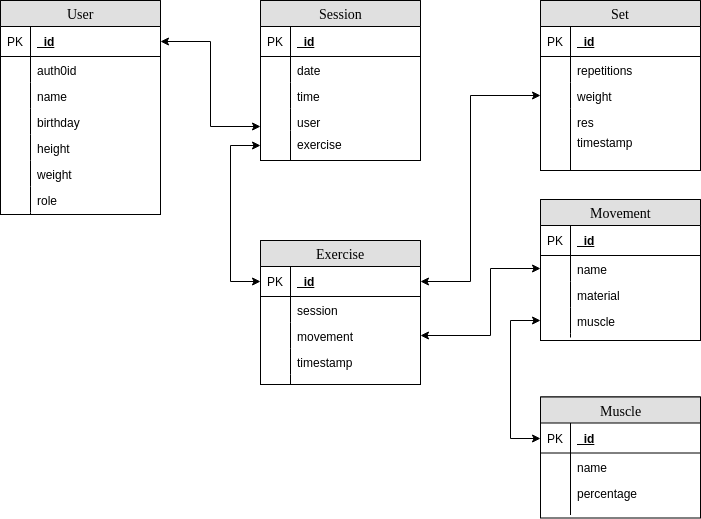
\includegraphics[width=\textwidth]{imagenes/db.png}
    \caption{Esquema base de datos}
    \label{fig:db}
  \end{center}
\end{figure}

\subsection {Diagrama conceptual}
En la imagen \ref{fig:esquema_alto_nivel} se muestra un diagrma simplificado del funcionamiento global de la aplicación.
\begin{figure}
  \begin{center}
    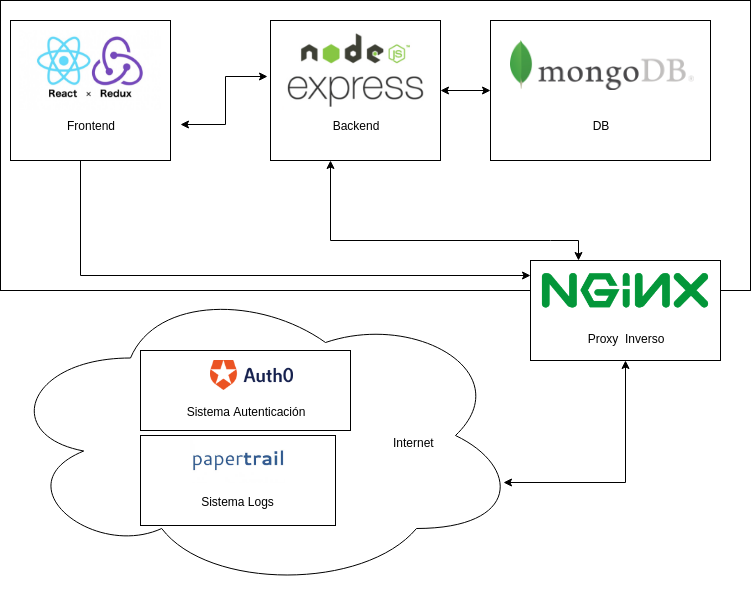
\includegraphics[width=\textwidth]{imagenes/diagrama_conceptual.png}
    \caption{Esquema alto nivel}
    \label{fig:esquema_alto_nivel}
  \end{center}
\end{figure}


\subsection {Diagrama de clases}
\subsection {Ciclo de vida componente}
En esta sesión se muestra un diagrama del funcionamiento de React \ref{fig:react}
\begin{figure}
  \begin{center}
    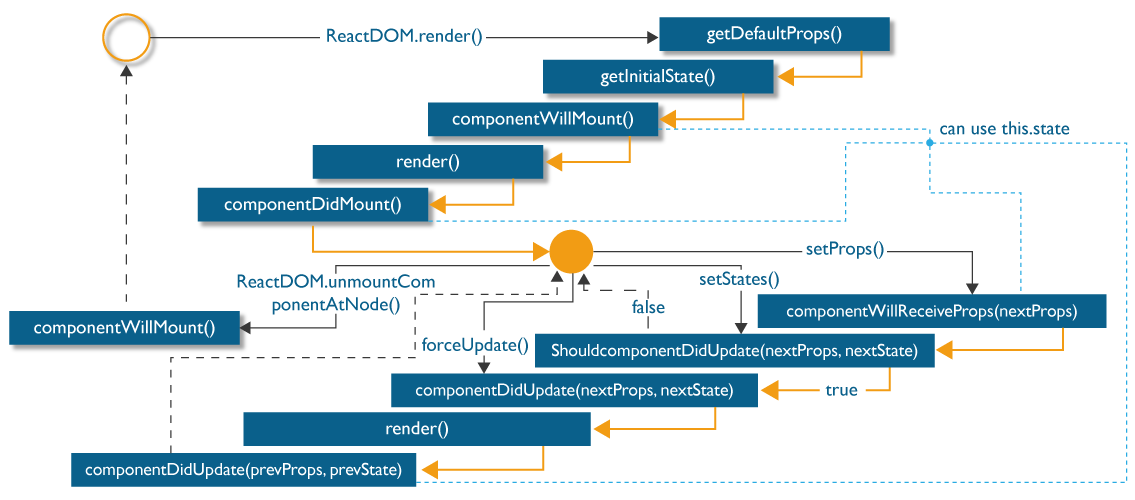
\includegraphics[width=\textwidth]{imagenes/ReactDOM_edureka.png}
    \caption{Ciclo de vida de un componente de React}
    \label{fig:react}
  \end{center}
\end{figure}

\subsection {React - Redux}
En esta sesión se muestra un diagrama del funcionamiento de React junto a Redux \ref{fig:react_redux}
\begin{figure}
  \begin{center}
    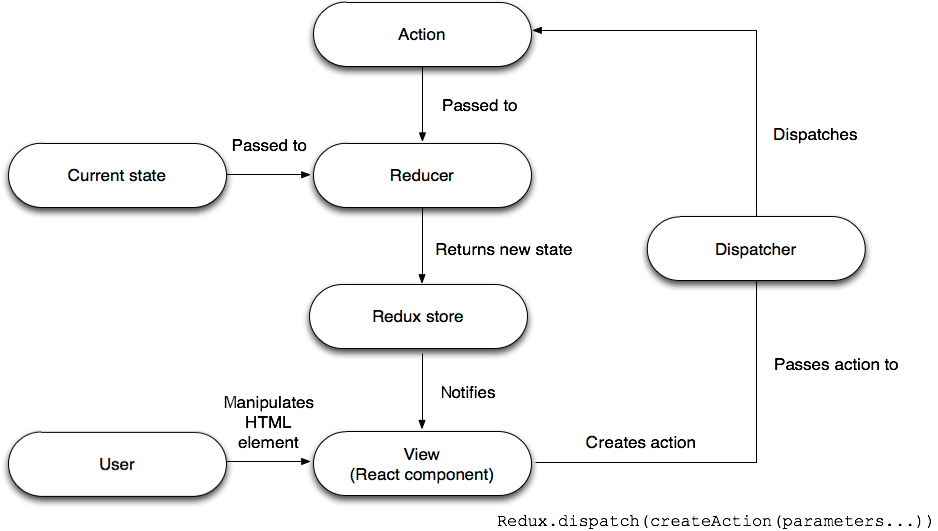
\includegraphics[width=\textwidth]{imagenes/react_redux.png}
    \caption{Diagrama React - Redux}
    \label{fig:react_redux}
  \end{center}
\end{figure}


  
